\chapter{Apartado A: \textbf{Sustracción de Fondo}}
\label{chapter:tarea_a}


\section*{Tarea A.1: Carga de vídeo}
\phantomsection
\addcontentsline{toc}{section}{Tarea A.1: Carga de vídeo}
Cargue el vídeo \texttt{'visiontraffic.avi'} en el cual se detectarán objetos en movimiento. Para ello, complete el método \texttt{read\_video} que podrá reutilizar en el resto de tareas. Utilizará la clase \texttt{VideoCapture} \footnote{ \href{https://docs.opencv.org/4.x/d8/dfe/classcv\_1\_1VideoCapture.html}{Documentación de la clase \texttt{VideoCapture} en OpenCV:} \\{https://docs.opencv.org/4.x/d8/dfe/classcv\_1\_1VideoCapture.html}} y sus métodos para gestionar la lectura del vídeo. Para obtener el ancho y alto de los fotogramas (y las FPS del vídeo), utilice la documentación de OpenCV \footnote{ \href{https://docs.opencv.org/4.x/d4/d15/group\_\_videoio\_\_flags\_\_base.html\#gaeb8dd9c89c10a5c63c139bf7c4f5704d}{Documentación de los argumentos \texttt{VideoCaptureProperties} en OpenCV:} \\{https://docs.opencv.org/4.x/d4/d15/group\_\_videoio\_\_flags\_\_base.html\#gaeb8dd9c89c10a5c63c139bf7c4f5704d}}.


\section*{Tarea A.2: Sustracción de fondo mediante diferencia de frames}
\phantomsection
\addcontentsline{toc}{section}{Tarea A.2: Sustracción de fondo mediante diferencia de frames}
Realice una sustracción de fondo mediante diferencia de frames, para ello guarde un frame con el fondo estático y úselo como frame de referencia de fondo.

En primer lugar vamos a iterar sobre la lista de frames para mostrar por pantalla frame a frame e iremos avanzando pulsando la tecla $n$, para seleccionar el frame de referencia deberá pulsar la tecla $s$.

Posteriormente se realizará la diferencia de frames entre el frame referencia y el frame actual.

\begin{figure}[H]
    \centering
    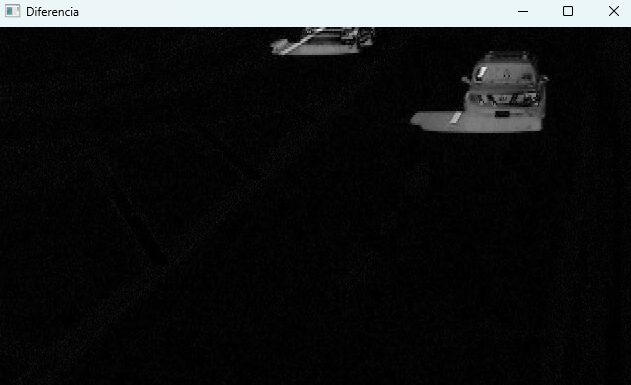
\includegraphics[width=0.4\textwidth]{Lab_4/template/figures/frame_difference.png}
    \caption{Ejemplo de resultado con diferencia de frames.}
    \label{fig:ejemplo_framediff}
\end{figure}

\section*{Tarea A.3: Configuración de la Sustracción de Fondo con GMM}
\phantomsection
\addcontentsline{toc}{section}{Tarea A.3: Configuración de la Sustracción de Fondo con GMM}

Configure el sustractor de fondo usando el modelo de mezcla de gaussianas adaptativas (MOG2). Para ello, usaremos \texttt{cv2.createBackgroundSubtractorMOG2}\footnote{ \href{https://docs.opencv.org/4.8.0/d7/d7b/classcv_1_1BackgroundSubtractorMOG2.html}{Documentación del método \texttt{MOG2} en OpenCV:} \\{https://docs.opencv.org/4.8.0/d7/d7b/classcv\_1\_1BackgroundSubtractorMOG2.html}}

\section*{Tarea A.4: Aplicación de la Sustracción de Fondo}
\phantomsection
\addcontentsline{toc}{section}{Tarea A.4: Aplicación de la Sustracción de Fondo}
Aplique la sustracción de fondo en cada frame para extraer los objetos en movimiento.


Visualice el resultado de la detección de movimiento y guarde el vídeo con las imagenes binarias resultantes en la carpeta \texttt{data/results}. Utilize el método \texttt{cv2.VideoWriter}\footnote{ \href{https://docs.opencv.org/4.8.0/dd/d9e/classcv_1_1VideoWriter.html}{Documentación del método \texttt{VideoWriter} en OpenCV:} \\{https://docs.opencv.org/4.8.0/dd/d9e/classcv\_1\_1VideoWriter.html}}

\begin{figure}[H]
    \centering
    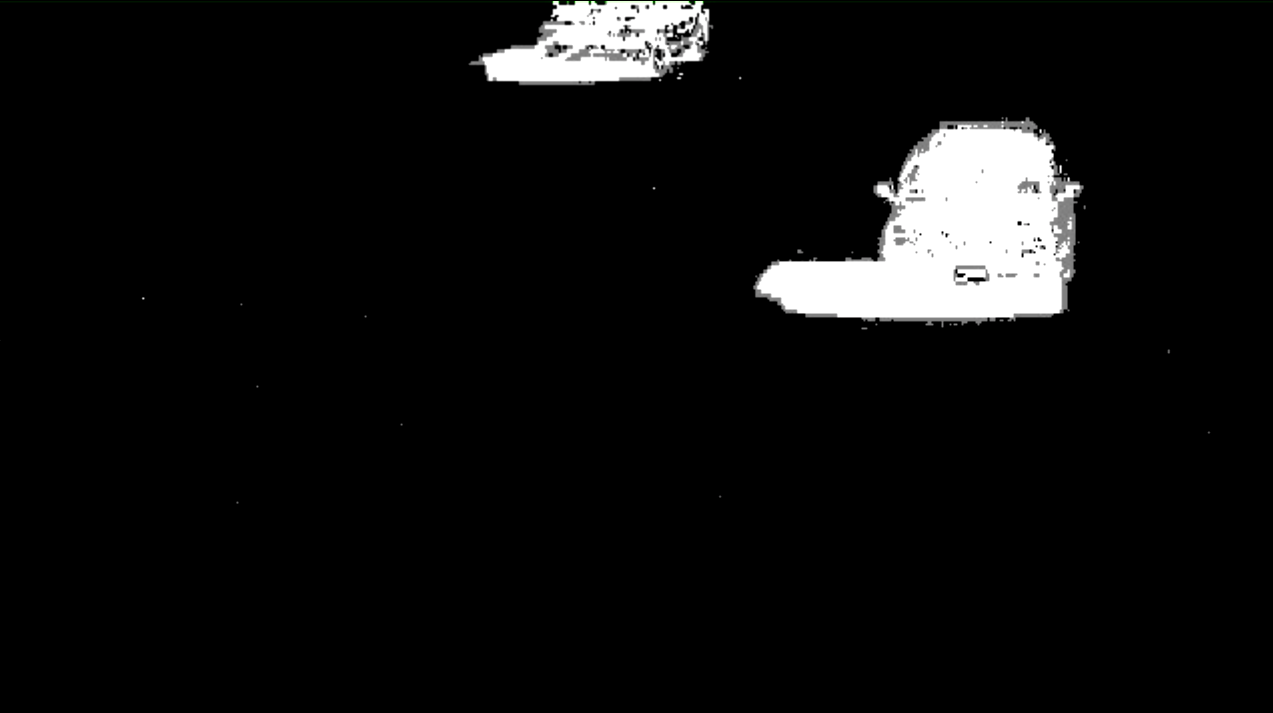
\includegraphics[width=0.4\textwidth]{Lab_4/template/figures/MOG2.png}
    \caption{Ejemplo de resultado usando MOG2.}
    \label{fig:ejemplo_mog2}
\end{figure}

\section*{Preguntas}
\addcontentsline{toc}{section}{Preguntas}

\vspace{5mm}
\begin{tcolorbox}[colback=gray!10, colframe=gray!30, coltitle=black, title=Pregunta A.1, halign=left]
¿Cómo afecta la variable \texttt{varThreshold} a la precisión de la detección?
\end{tcolorbox}

\vspace{5mm}
\begin{tcolorbox}[colback=gray!10, colframe=gray!30, coltitle=black, title=Pregunta A.2, halign=left]
¿Qué ventajas presenta \texttt{createBackgroundSubtractorMOG2} frente a métodos simples de diferencia de imágenes?
\end{tcolorbox}